%%%%%%%%%%%%%%%%%%%%%%%%%%%%%%%%%%%%%%%%%%%%%%%%%%%%%%
% A Beamer template for University of Wollongong     %
% Based on THU beamer theme                          %
% Author: Qiuyu Lu                                   %
% Date: July 2024                                    %
% LPPL Licensed.                                     %
%%%%%%%%%%%%%%%%%%%%%%%%%%%%%%%%%%%%%%%%%%%%%%%%%%%%%%
% Customized for Sharif University of Technology     %
%%%%%%%%%%%%%%%%%%%%%%%%%%%%%%%%%%%%%%%%%%%%%%%%%%%%%%


\documentclass[default, aspectratio=169]{beamer}
%\documentclass[default]{beamer}  % for 4:3 ratio
\usepackage[T1]{fontenc} 
\usepackage{fourier} % see "http://faq.ktug.org/wiki/uploads/MathFonts.pdf" for other options
\usepackage{hyperref}
\usepackage{latexsym,amsmath,xcolor,multicol,booktabs,calligra}
\usepackage{graphicx,pstricks,listings,stackengine}
\usepackage{lipsum}

\author{Ali Sharifi-Zarchi}
\title{Machine Learning (CE 40717)}
\subtitle{Fall 2024}
\institute{
	CE Department \\
	Sharif University of Technology
}
%\date{\small \today}
% \usepackage{UoWstyle}
\usepackage{SUTstyle}
\usepackage{amsmath}
\usepackage{amssymb}
% defs
\def\cmd#1{\texttt{\color{red}\footnotesize $\backslash$#1}}
\def\env#1{\texttt{\color{blue}\footnotesize #1}}
\definecolor{deepblue}{rgb}{0,0,0.5}
\definecolor{deepred}{RGB}{153,0,0}
\definecolor{deepgreen}{rgb}{0,0.5,0}
\definecolor{halfgray}{gray}{0.55}

\lstset{
	basicstyle=\ttfamily\small,
	keywordstyle=\bfseries\color{deepblue},
	emphstyle=\ttfamily\color{deepred},    % Custom highlighting style
	stringstyle=\color{deepgreen},
	numbers=left,
	numberstyle=\small\color{halfgray},
	rulesepcolor=\color{red!20!green!20!blue!20},
	frame=shadowbox,
}

\begin{document}


	
	\begin{frame}
		\titlepage
		\vspace*{-0.6cm}
		\begin{figure}[htpb]
			\begin{center}
				
\includegraphics[keepaspectratio, scale=0.25]{pic/sharif-main-logo.png}
			\end{center}
		\end{figure}
	\end{frame}
	
	\begin{frame}    
		\tableofcontents[sectionstyle=show,
		subsectionstyle=show/shaded/hide,
		subsubsectionstyle=show/shaded/hide]
	\end{frame}
	
	\section{Motivation}
	\begin{frame}{How do humans see?}
		
		\begin{center}
			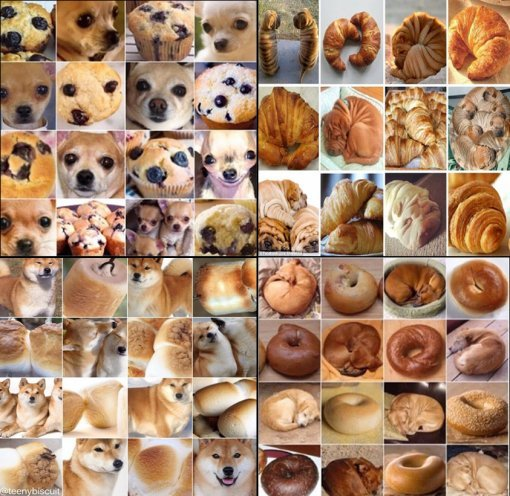
\includegraphics[keepaspectratio, scale=0.334]{pic/how.png}
			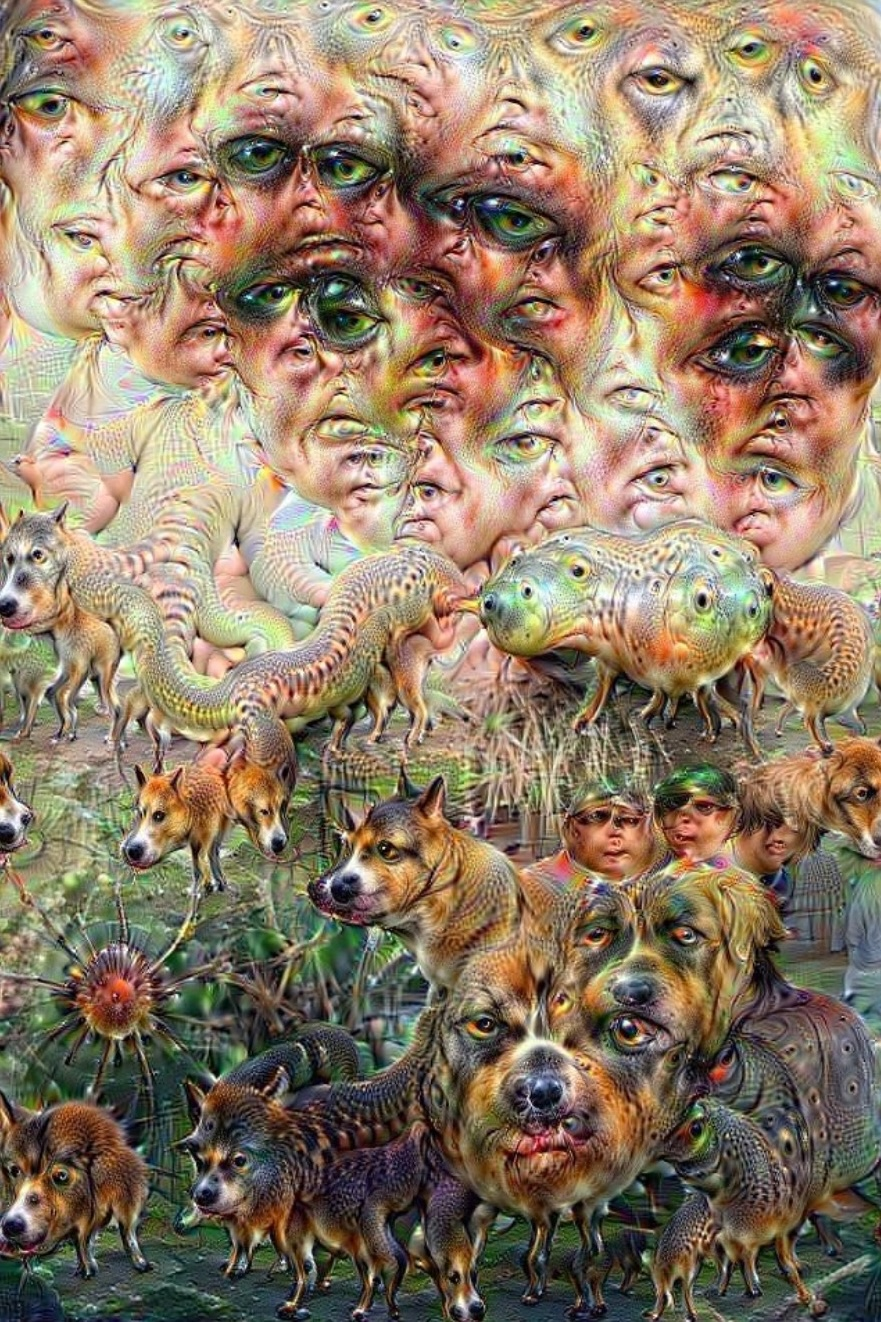
\includegraphics[keepaspectratio, scale=0.25]{pic/nothing.PNG}
		\end{center}
		How can we enable computers to see?
	\end{frame}
	\begin{frame}{What computers ‘see’: images as numbers}
		\centering
		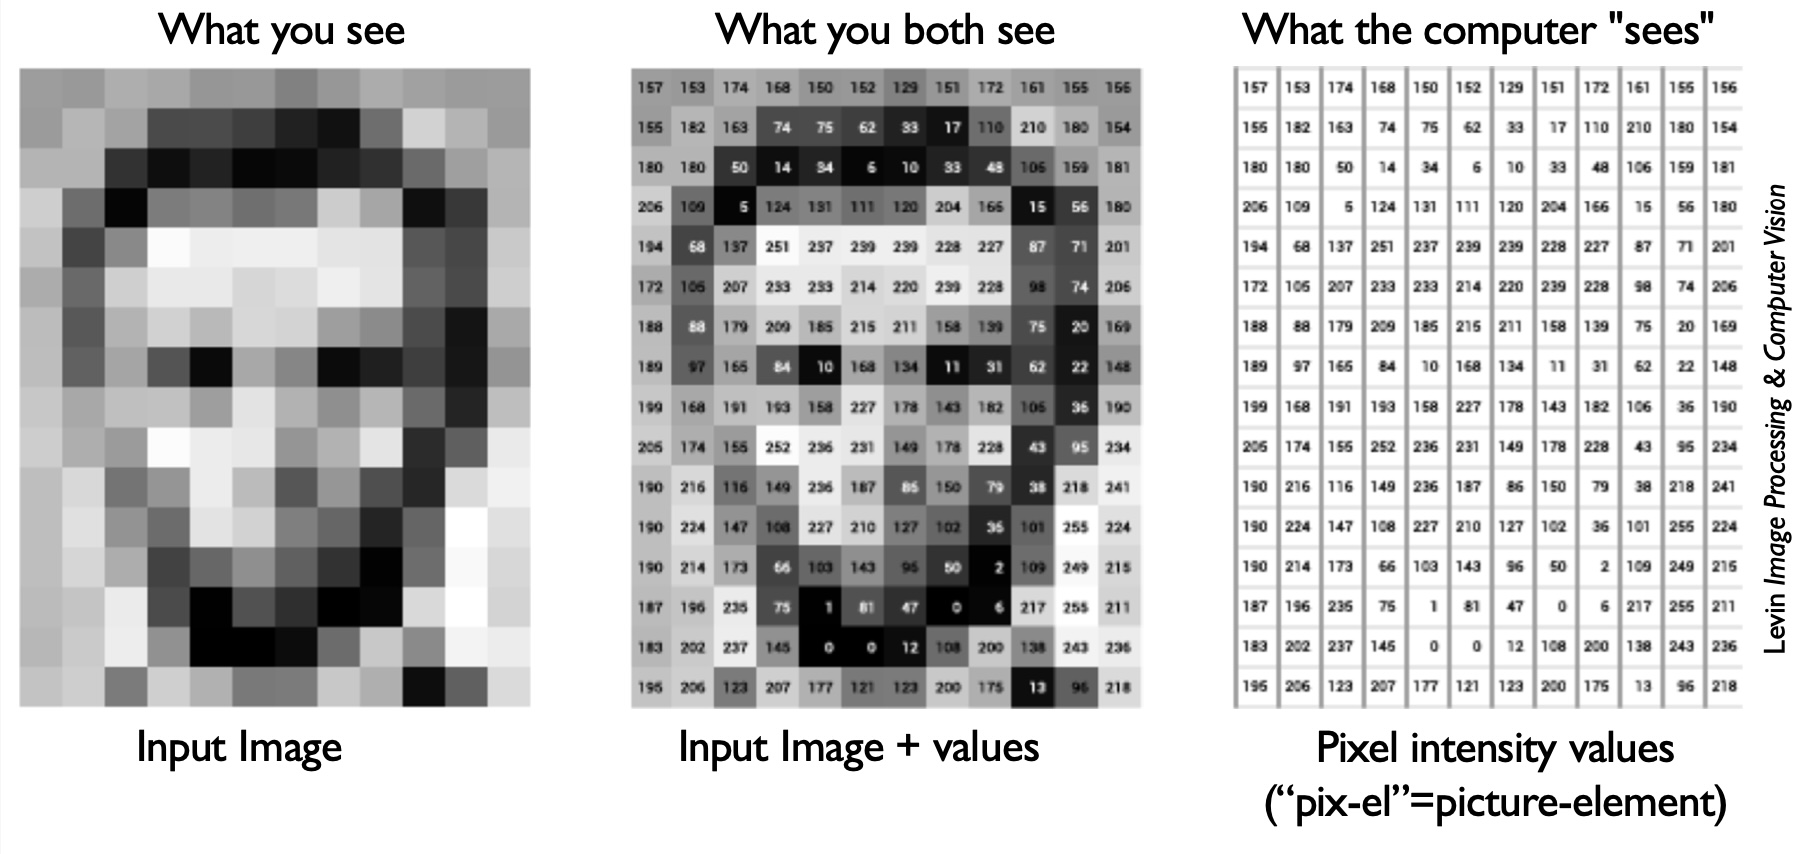
\includegraphics[keepaspectratio, scale=0.35]{pic/what.png}
		\\{An image is just a matrix of numbers [0,255].i.e., $1080 \times 1080 \times 3$ for an RGB image.\\ Question: is this Lincoln? Washington? Jefferson? Obama?
			How can the computer answer this question?}
	\end{frame}
	\begin{frame}{What is computer vision? (1)}
		\centering
		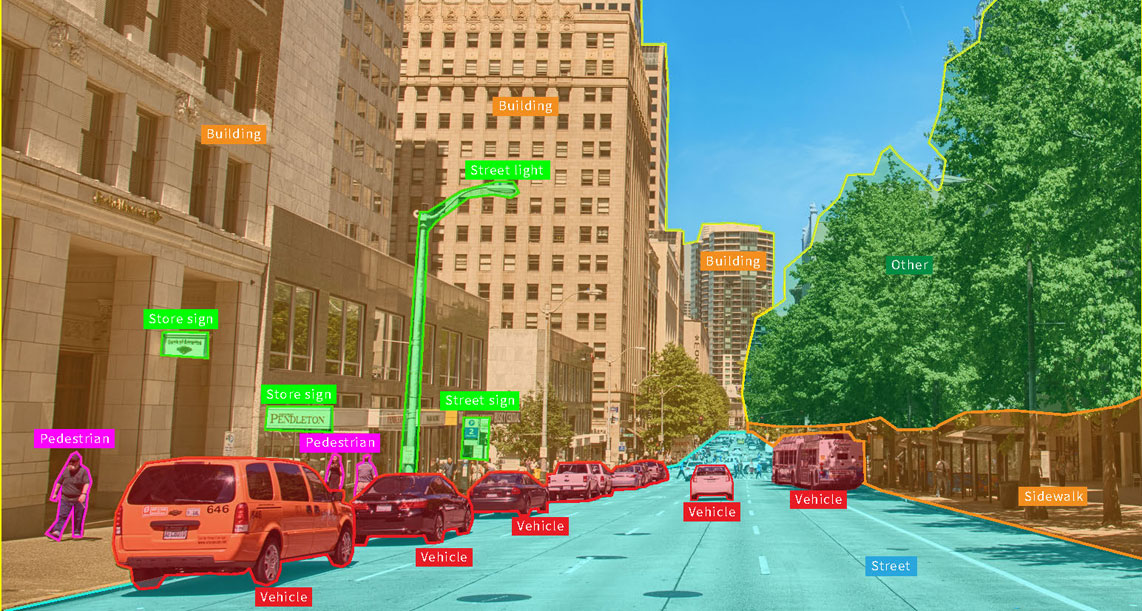
\includegraphics[keepaspectratio, scale=0.3]{pic/computer_vision.jpeg}		
		
	\end{frame}
	\begin{frame}{What is computer vision? (2)}
		\centering
		\begin{minipage}{0.45\textwidth}
			\centering
			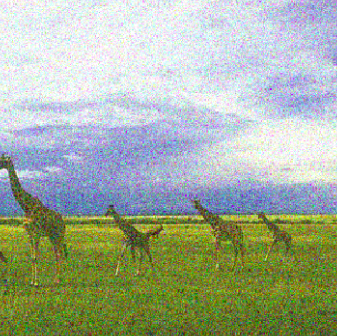
\includegraphics[width=\textwidth, keepaspectratio]{pic/noisy_image.png}
			\\Noisy Image
		\end{minipage}%
		\hspace{0.05\textwidth} % Adjusts space between the two images
		\begin{minipage}{0.45\textwidth}
			\centering
			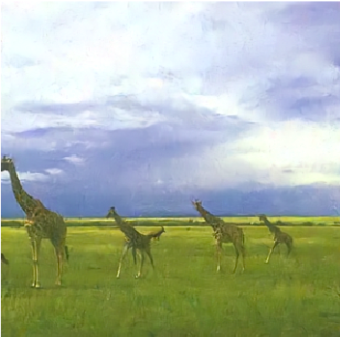
\includegraphics[width=\textwidth, keepaspectratio]{pic/denoised_image.png}
			\\Denoised Image
		\end{minipage}
	\end{frame}
	\begin{frame}{What is computer vision? (3)}
		\centering
		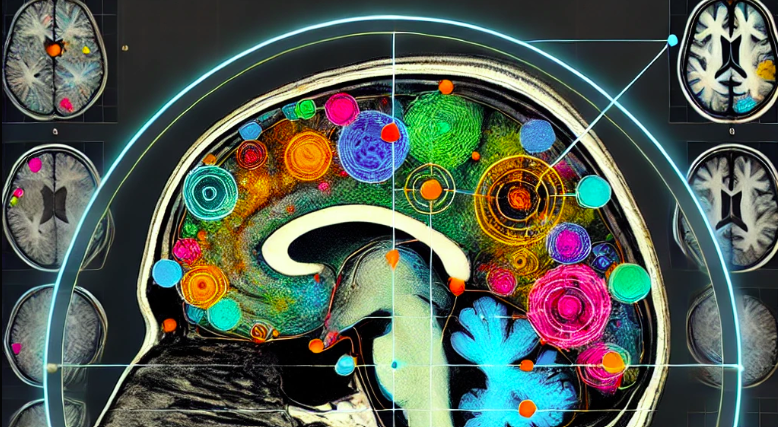
\includegraphics[keepaspectratio, scale=0.7]{pic/medical.png}		
	\end{frame}
	\begin{frame}{Hand-crafted features: before deep learning features (1)}
		\centering
		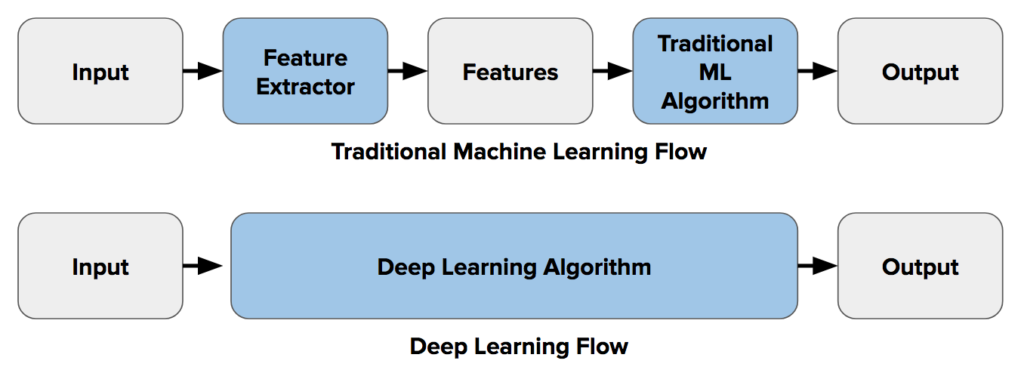
\includegraphics[keepaspectratio, scale=0.44]{pic/handcrafted_features.png}\\
		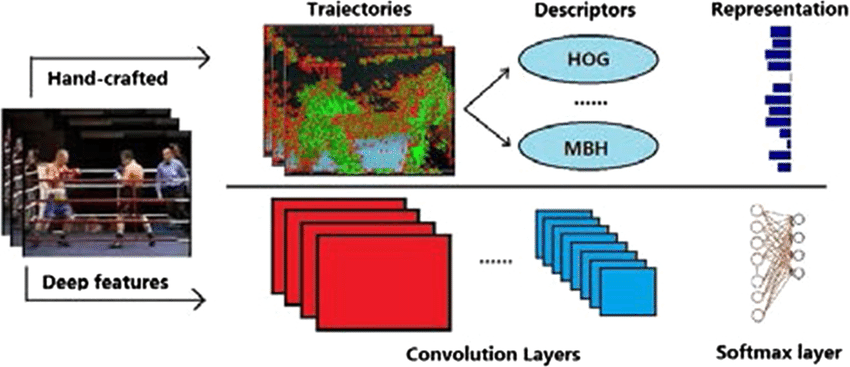
\includegraphics[keepaspectratio, scale=0.27]{pic/Two-types-of-features-used-for-action-recognition-ie-hand-crafted-features-and-deep.png}
		\\ \small {Two types of features used for action recognition, i.e., hand-crafted features and deep learning features
		}
	\end{frame}
	\begin{frame}{Hand-crafted features: before deep learning features (2)}
		\centering
		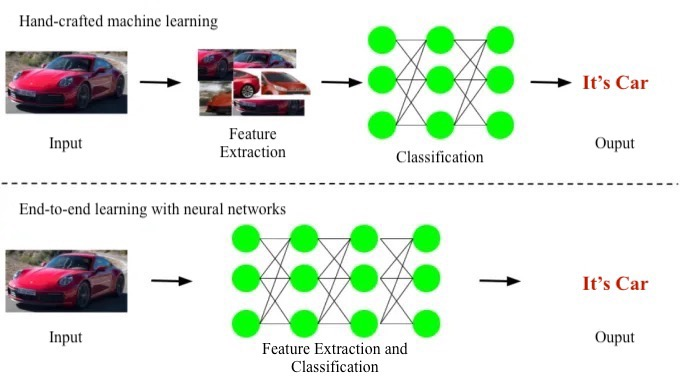
\includegraphics[keepaspectratio, scale=0.5]{pic/do-machine-learning-neural-networks-tasks-using-python copy 3.jpg}
	\end{frame}
	\begin{frame}{Image features}
		\centering
		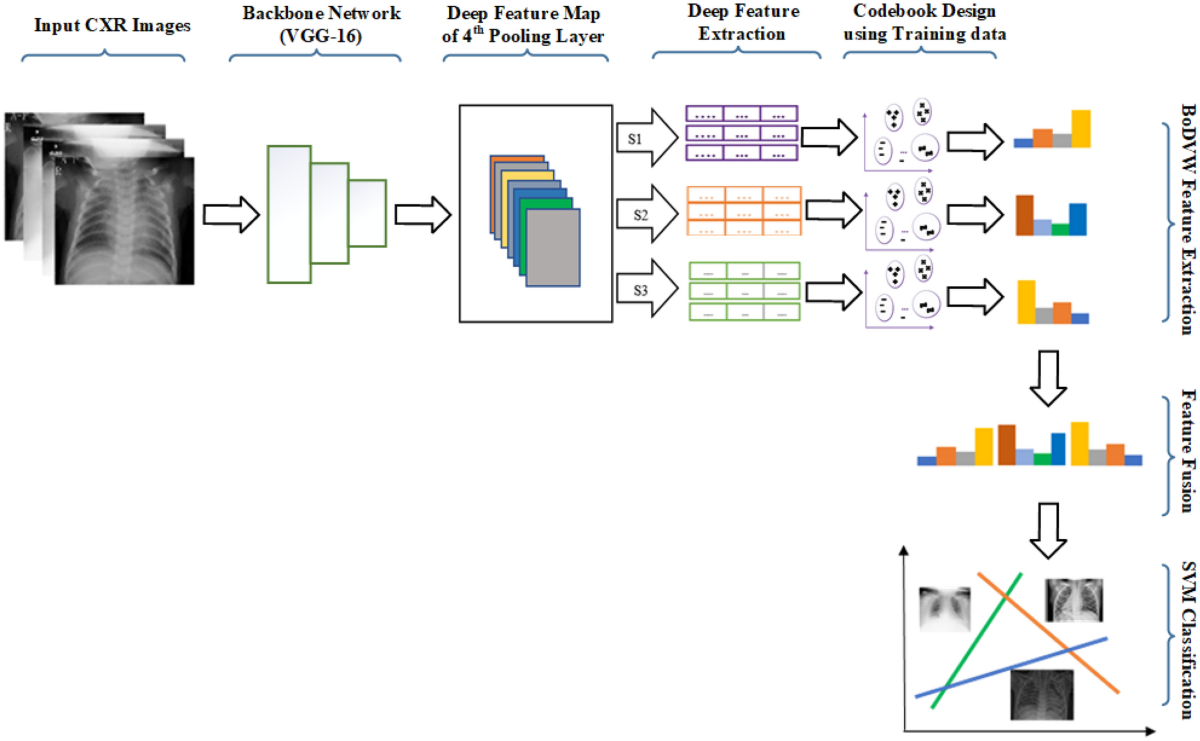
\includegraphics[keepaspectratio, scale=0.23]{pic/image_features.png}\\ \small{Fusion of multi-scale bag of deep visual words features of chest X-ray images to detect COVID-19 infection}
	\end{frame}
	\begin{frame}{Effect of dl}
		\centering
		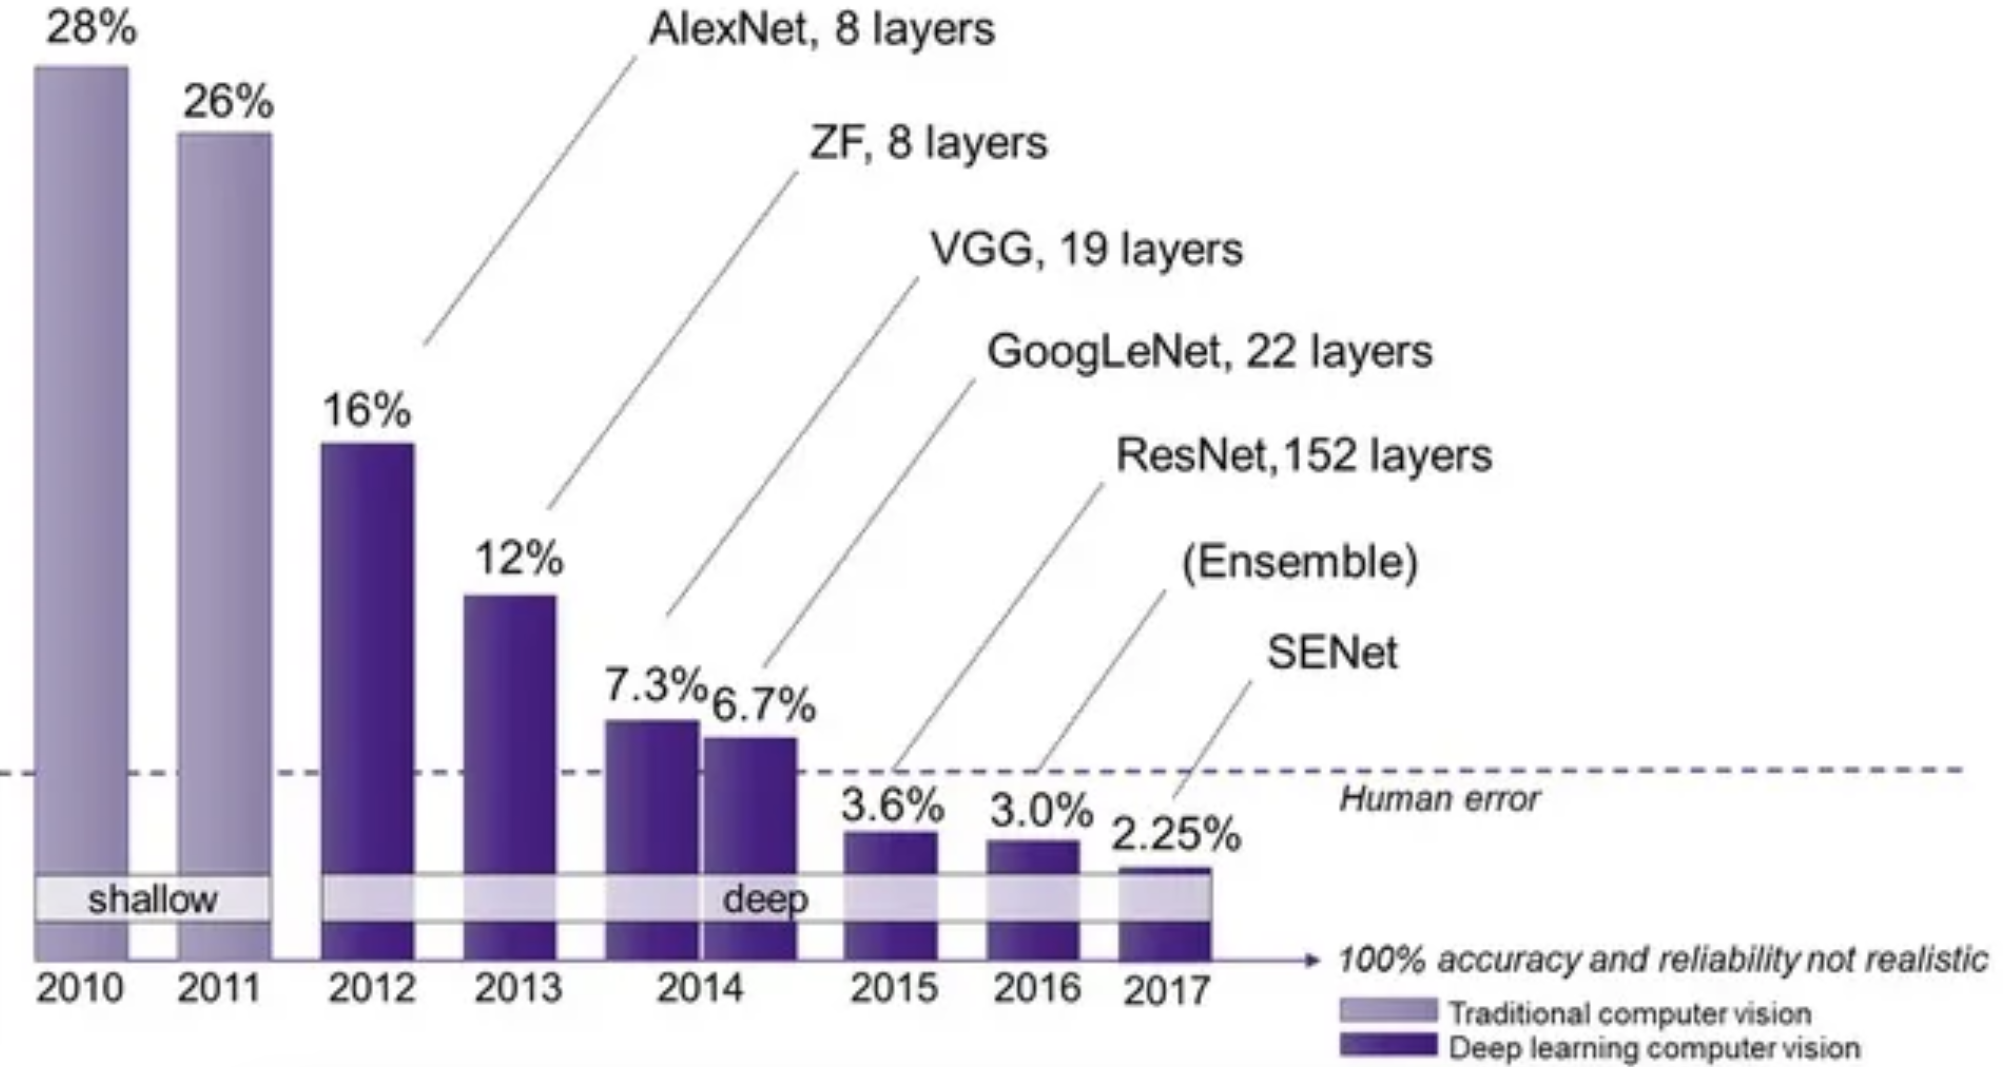
\includegraphics[keepaspectratio, scale=0.35]{pic/Synopsys_computer-vision-processors.png}\\\small{Comparison between Deep Learning and Traditional Models}
	\end{frame}
	
	
	
	\section{CNN vs. FCN}
	\begin{frame}{FCNs on images}
		\textcolor{red}{Dense} Vector Multiplication
		\begin{center}
			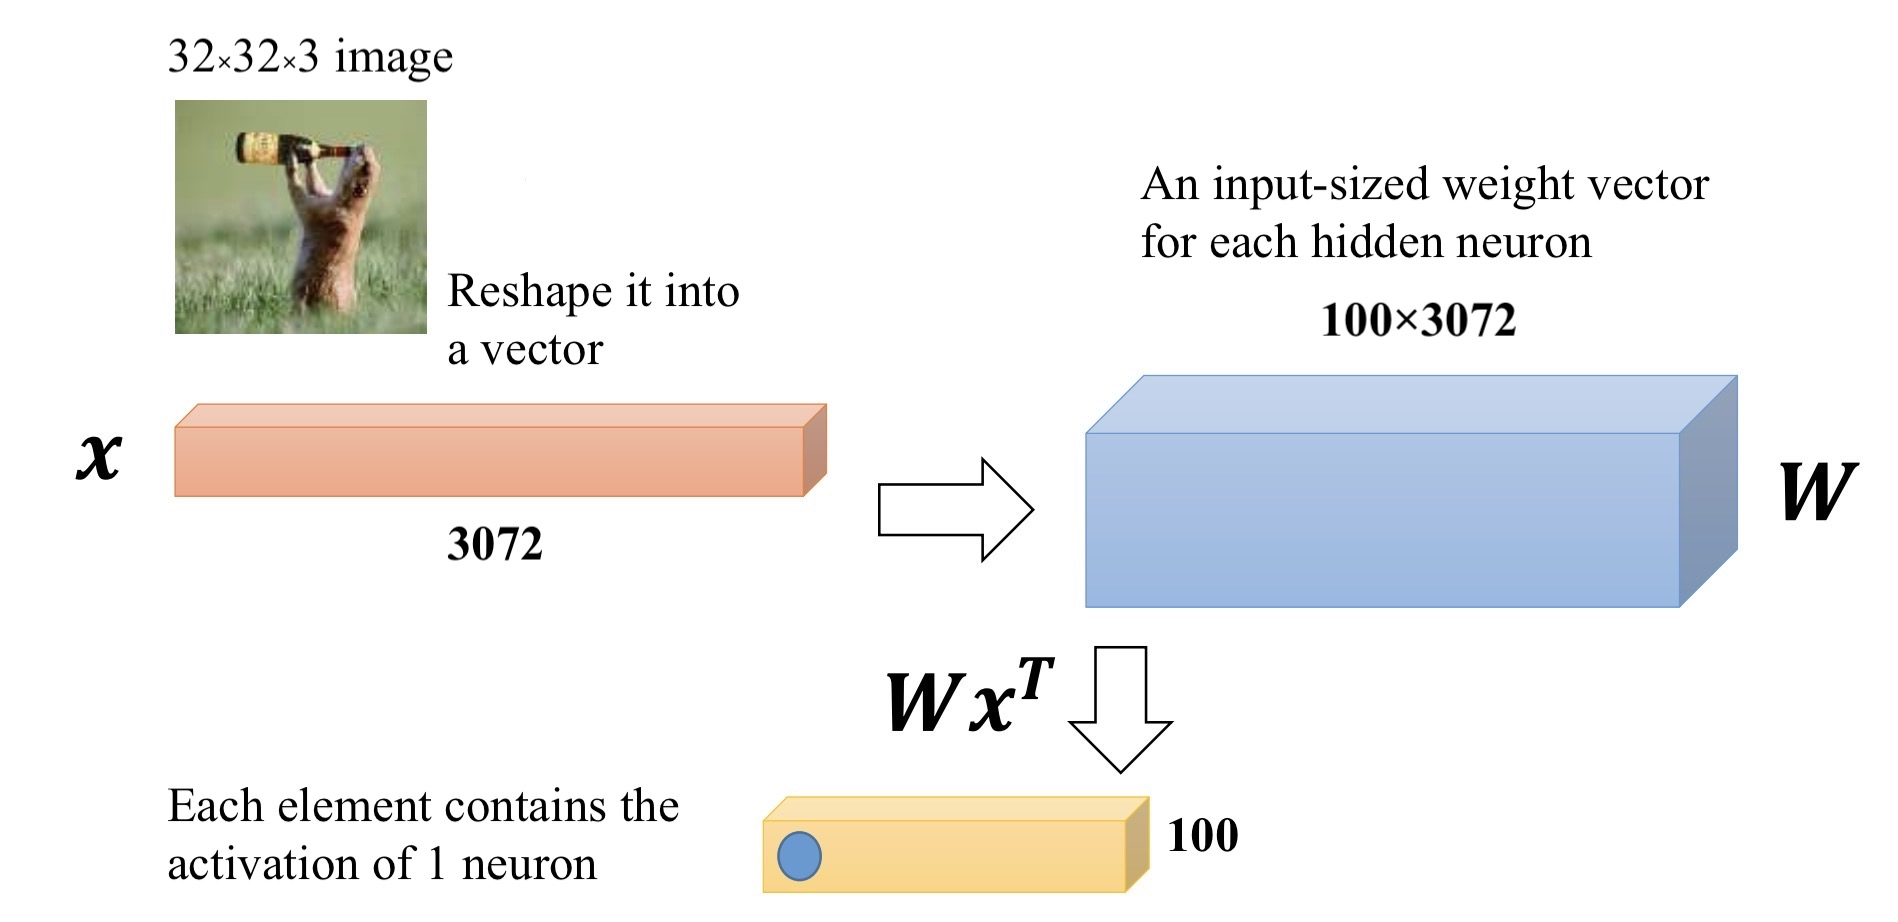
\includegraphics[keepaspectratio, scale=0.2]{pic/Processing images.jpg}
		\end{center}
	\end{frame}
	\begin{frame}{Fully connected layers}
		\begin{itemize}
			\item Neurons in a single layer operate independently and do not share connections, even for inputs.
			
			\bigskip
			
			\item To be shift-invariant, many samples (in various time or locations) must be shown to them.
			
			\bigskip
			
			\item \textbf{Regular Neural Nets don’t scale well to full images}
			\begin{itemize}
				\item Parameters would add up quickly!
				\item Full connectivity is wasteful and the huge number of parameters would quickly lead to overfitting.
			\end{itemize}
		\end{itemize}
	\end{frame}
	\begin{frame}{Invariance vs equivariance}
		\begin{center}
			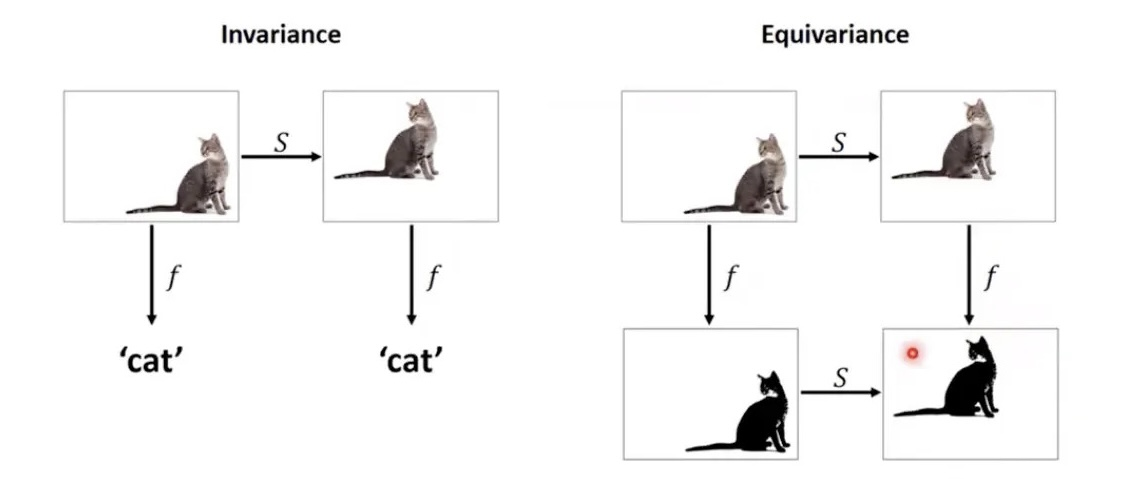
\includegraphics[keepaspectratio, scale=0.28]{pic/invariance_vs_equivariance.jpg}
		\end{center}
		\begin{itemize}
			\item \textbf{Invariance:} The output remains the same when the input undergoes a transformation.
			\item \textbf{Equivariance:} The output varies predictably when the input undergoes a transformation.
			
		\end{itemize}
	\end{frame}
	\begin{frame}{Shift-invariance}
		\begin{center}
			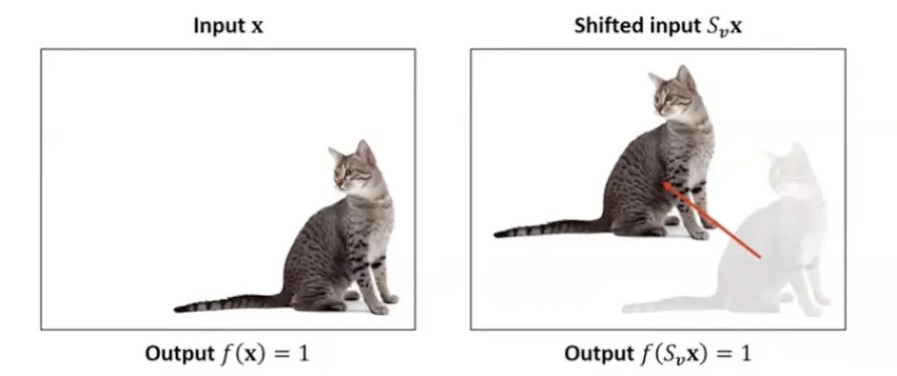
\includegraphics[keepaspectratio, scale=0.25]{pic/shift_invariance.jpg}
		\end{center}
		
		\begin{itemize}
			\item \textit{Cat detector} \quad $f: \mathbb{R}^d \to \mathbb{R}$
			
			\item \textit{Shift operator} \quad $S_v: \mathbb{R}^d \to \mathbb{R}^d$ \quad shifting the image by vector $v$
		\end{itemize}
		
		\textbf{Shift invariance:} \quad $f(\mathbf{x}) = f(S_v \mathbf{x})$ 
		\\ \textcolor{red}{Will an MLP that recognizes the left image as a cat also recognize the shifted image on the right as a cat?}
	\end{frame}
	\begin{frame}{A problem}
		\begin{itemize}
			\item In many problems the \textit{location} of a pattern is not important
			\begin{itemize}
				\item Only the presence of the pattern matters matters
			\end{itemize}
			\item Traditional MLPs are sensitive to pattern location
			\begin{itemize}
				\item Moving it by one component results in an entirely different input that the MLP won’t recognize
			\end{itemize}
			
			\item \textbf{Requirement:} Network must be \textit{shift invariant}
		\end{itemize}
	\end{frame}
	\begin{frame}{Convolution on images}
		Convolution (Refresher)
		\begin{center}
			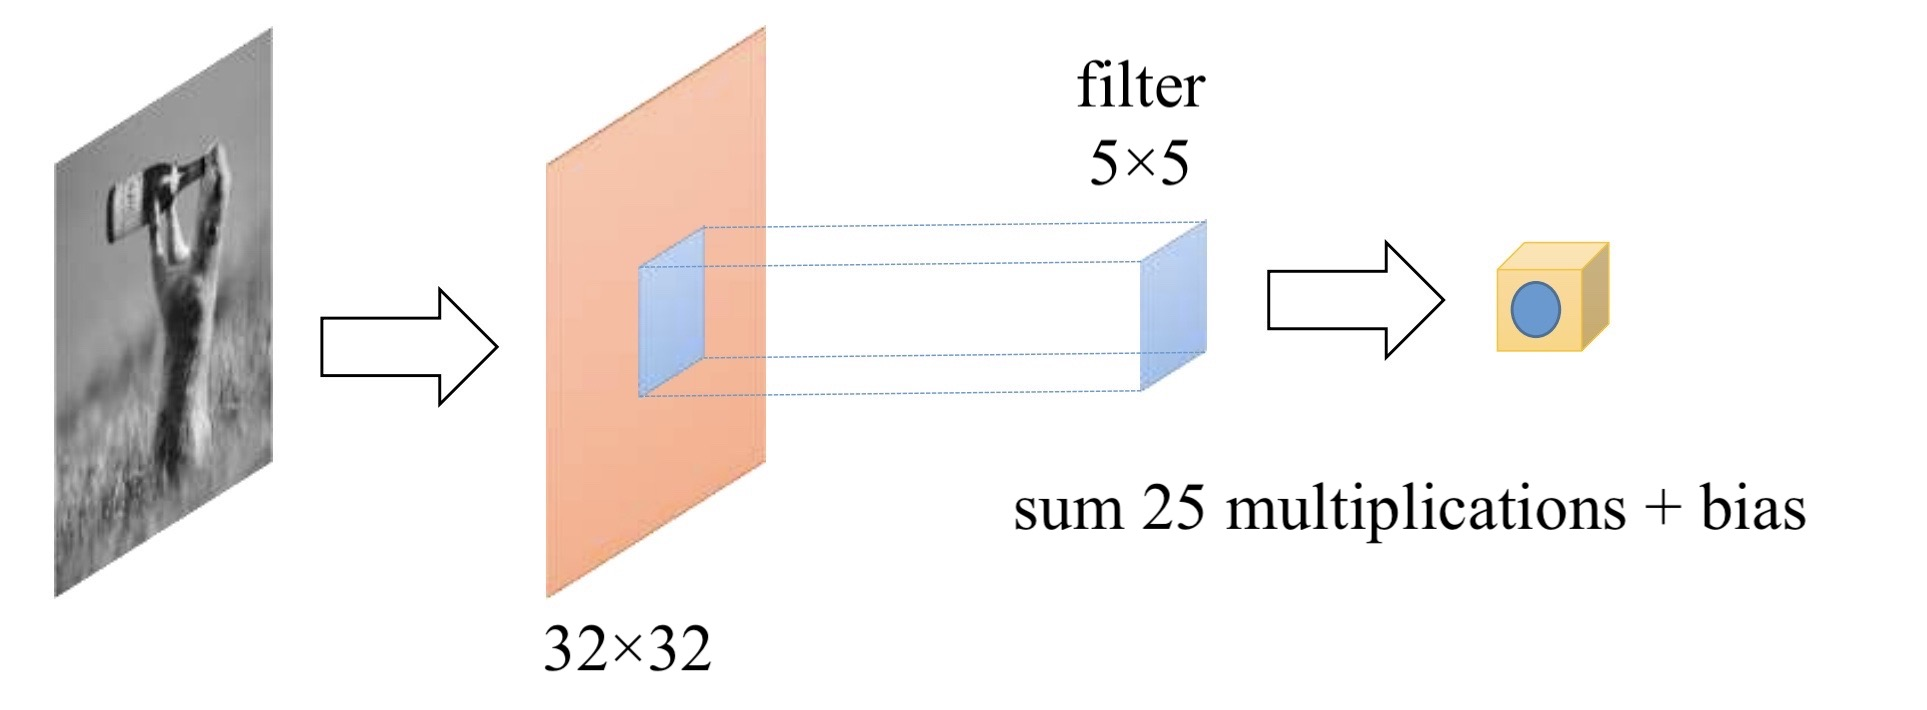
\includegraphics[keepaspectratio, scale=0.2]{pic/conv.jpg}
			
			Matrix input preserving \textcolor{red}{spatial structure}
		\end{center}
		
	\end{frame}
	\begin{frame}{Fully connected or convolution}
		
		\textbf{Question:}
		Can I just do classification on an flatten image (e.g., a 1080x1080x3 image) with fully connected layers?
		
		\bigskip
		
		\textbf{Answer:} 
		No, using fully connected layers on such a large image is inefficient due to:
		\begin{itemize}
			\item Loss of spatial structure
			\item High parameter count
		\end{itemize}
		
		\bigskip
		
		\textbf{Why Use Convolution:}
		\begin{itemize}
			\item \textbf{Exploit spatial structure:} Convolution sees local patterns by using filters over small patches of the image.
			\item \textbf{Reduce parameters:} By sharing weights across the image, convolution reduce the number of parameters.
			\item \textbf{Build hierarchical features:} Convolution starts with small patterns, then combines them to recognize more complex patters.
		\end{itemize}
		
	\end{frame}	
	\begin{frame}{What is cnn?}
		\begin{itemize}
			\item It is a class of deep learning.
			
			\item Convolutional neural network (ConvNet’s or CNNs) is one of the main categories to do image recognition, image classifications, object detection, recognition of faces, etc.
			
			\item It is similar to the basic neural network. CNNs also have learnable parameters like weights and biases, similar to neural networks.
			
			\item CNN is heavily used in computer vision.
			
			\item There are 3 basic components to define CNN:
			\begin{itemize}
				\item The Convolution Layer
				\item The Pooling Layer
				\item The Output Layer (or) Fully Connected Layer
			\end{itemize}
		\end{itemize}
		
	\end{frame}
	\begin{frame}{Architecture of CNN}
		\centering
		The basic idea of Convolutional Neural Networks (CNNs) is similar to Backpropagation Neural Networks (BPNNs) but differs in implementation.
		
		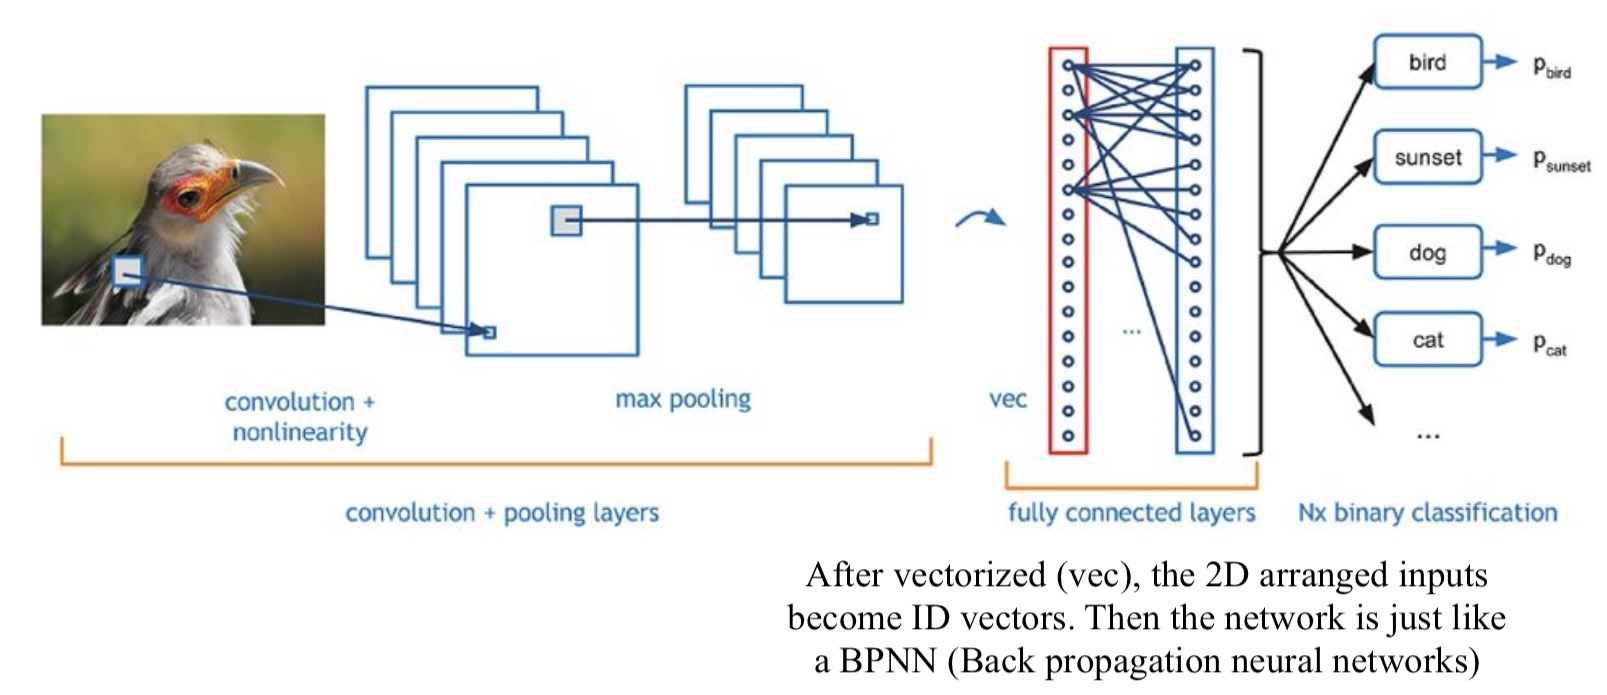
\includegraphics[keepaspectratio, scale=0.5]{pic/Architecture_of_CNN.jpg}
	\end{frame}
	\begin{frame}{The basic structure (1)}
		\begin{itemize}
			\item Alternating \textcolor{red}{Convolution (C)} and \textcolor{red}{subsampling layer (S)}
			\item Subsampling allows flexible positioning of features.
		\end{itemize}
		\begin{center}
			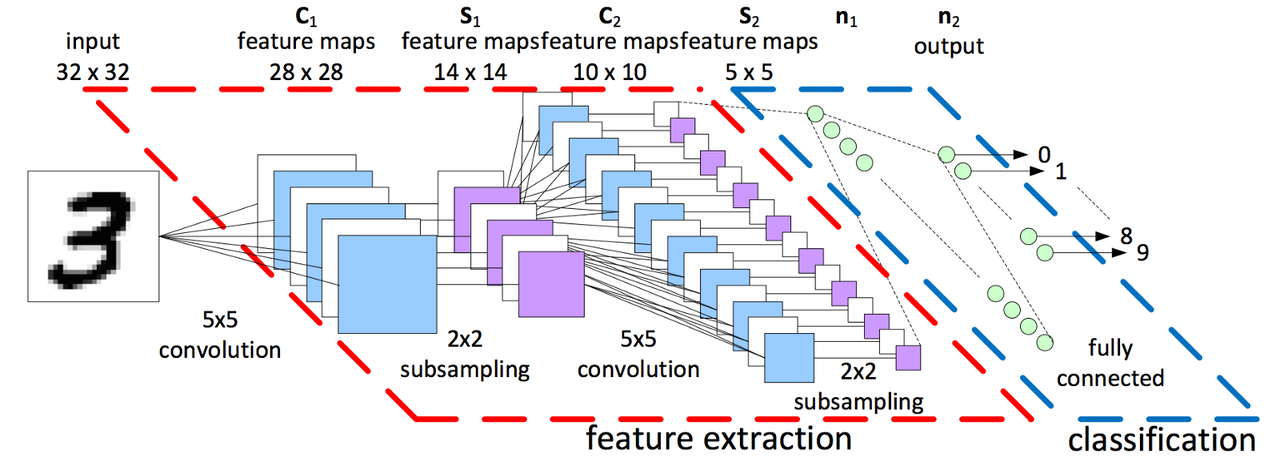
\includegraphics[keepaspectratio, scale=0.23]{pic/CNN_structure_3.png}
		\end{center}
	\end{frame}
	\begin{frame}{The basic structure (2)}
		\begin{center}
			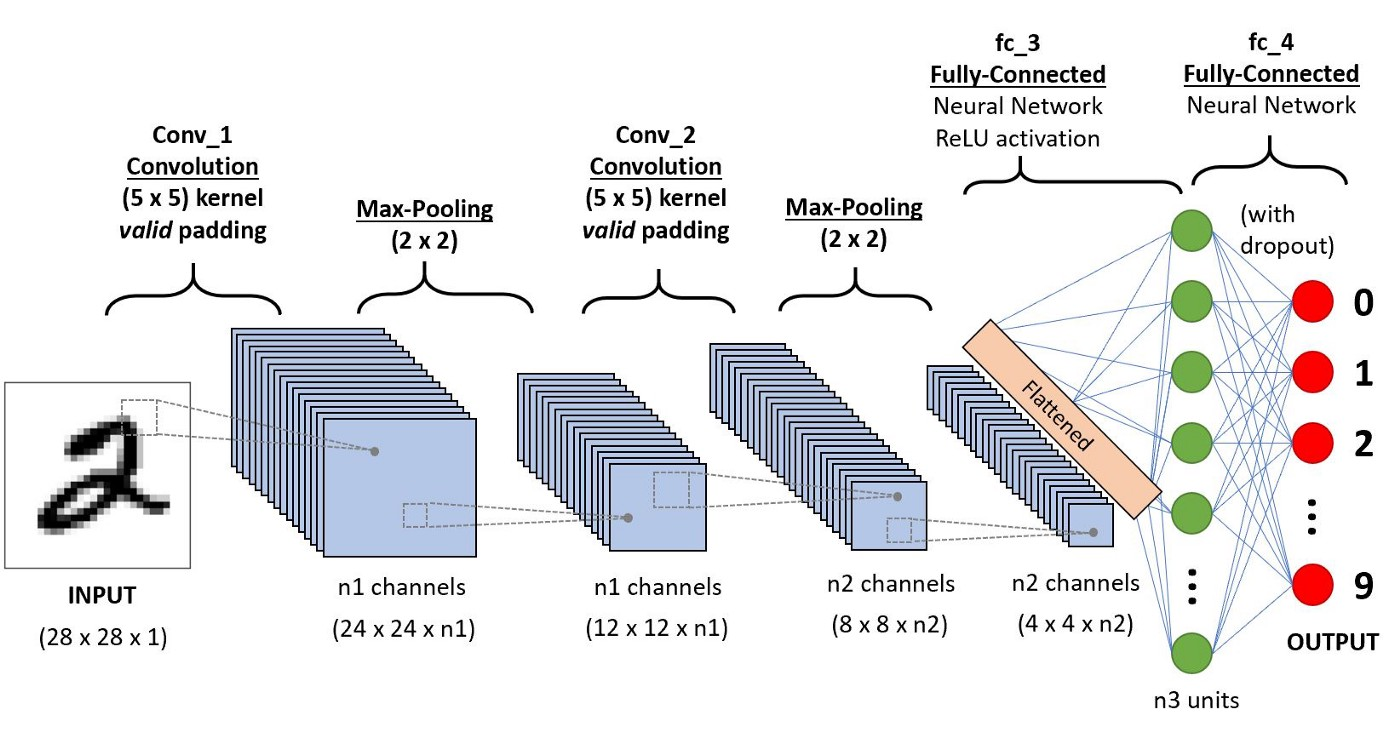
\includegraphics[keepaspectratio, scale=0.25]{pic/CNN_structure_a.jpeg}
		\end{center}
	\end{frame}
	\begin{frame}{The basic structure (3)}
		\item \textbf{Three Main Types of Layers}
		\begin{itemize}
			\item \textbf{Convolutional Layer}
			\begin{itemize}
				\item Output of neurons are connected to local regions in the input.
				\item Applying the same filter across the entire image.
				\item CONV layer’s parameters consist of a set of learnable filters.
			\end{itemize}
			\item \textbf{Pooling Layer}
			\begin{itemize}
				\item Performs a downsampling operation along the spatial dimensions.
			\end{itemize}
			\item \textbf{Fully-Connected Layer}
			\begin{itemize}
				\item Typically used in the final stages of the network to combine high-level features and make predictions.
			\end{itemize}
		\end{itemize}
	\end{frame}
	\begin{frame}{Cnn vs. FCN}
		\begin{itemize}
			\item \textbf{Fully Connected Networks (FCNs):}
			\begin{itemize}
				\item High number of parameters, leading to overfitting on large inputs (e.g., images).
				\item Lack of spatial awareness, making it sensitive to the exact positioning of patterns.
				\item Suitable for structured data but inefficient for image processing.
				
			\end{itemize}
			
			\item \textbf{Convolutional Neural Networks (CNN):}
			\begin{itemize}
				\item Uses filters to process only small parts of the input at a time (locality).
				\item Weight sharing and local connectivity reduce the number of parameters.
				\item Can recognize patterns independent of their location within the image (shift invariance).
				\item Efficient for image, video, and speech data.				
			\end{itemize}
			
		\end{itemize}
	\end{frame}
	
	
	\section{Convolution}
	\begin{frame}{What is a convolve}
		\centering
		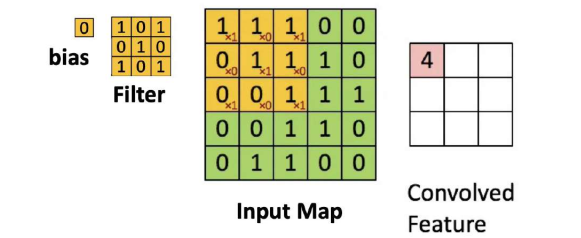
\includegraphics[keepaspectratio, scale=0.9]{pic/convo.png}
		\\
		\textbf{Scanning an image with a "filter"}
		
		\begin{itemize}
			\item A filter is really just a perceptron, with weights and a bias.
			\item At each location, the filter is multiplied component-wise with the underlying map values, and the products are summed along with the bias.
		\end{itemize}
		
	\end{frame}
	\begin{frame}{Weights showing correlation}
		\centering
		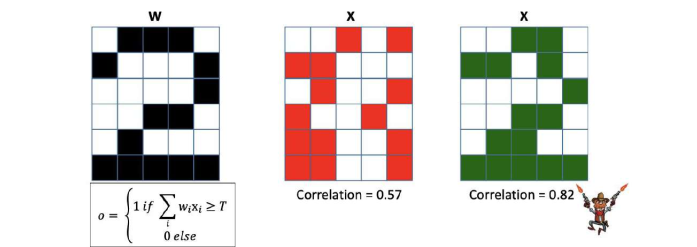
\includegraphics[keepaspectratio, scale=0.9]{pic/corr.png}
		\definecolor{darkgreen}{rgb}{0.0, 0.5, 0.0}
		\begin{itemize}
			\item The weights of the filter represent the appearance of the number "2".
			\item The \textcolor{deepgreen}{green} has a higher correlation with the filter compared to the \textcolor{red}{red}.
			\item The \textcolor{deepgreen}{green pattern} is more likely to represent the number "2".
		\end{itemize}
	\end{frame}
	\begin{frame}{What is convolution}
		\centering
		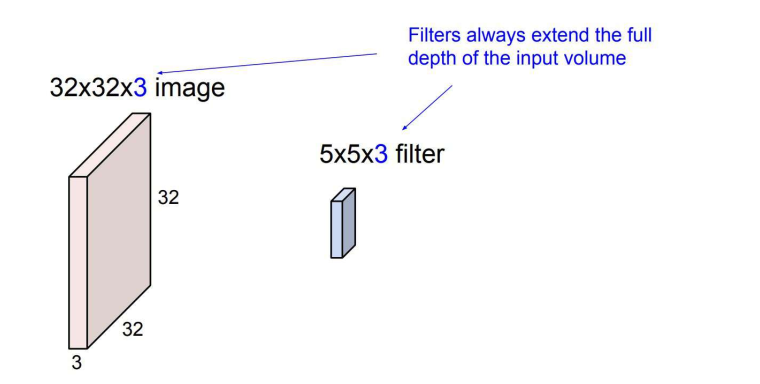
\includegraphics[keepaspectratio, scale=0.5]{pic/img.png}
		
		\smallskip
		\begin{itemize}
			\item \textbf {Convolve:} Slide over the image spatially, computing dot products.
			\item This allows us to preserve the spatial structure of the input.
		\end{itemize}
		
	\end{frame}
	\begin{frame}{What is the output}
		\centering
		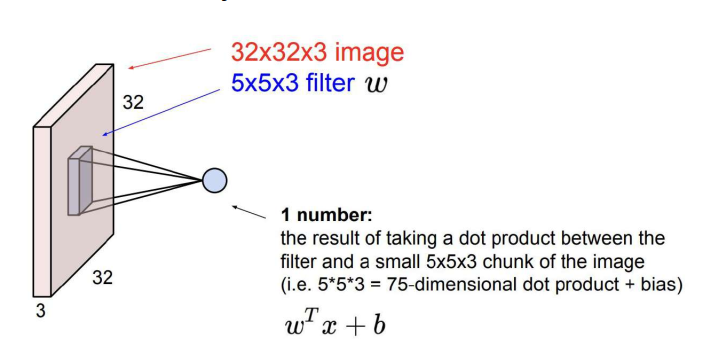
\includegraphics[keepaspectratio, scale=0.8]{pic/img1.png}	
		\begin{flushleft}
			It's simply a neuron with local connectivity!
		\end{flushleft}
	\end{frame}
	\begin{frame}{Convolution process (1)}
		\centering
		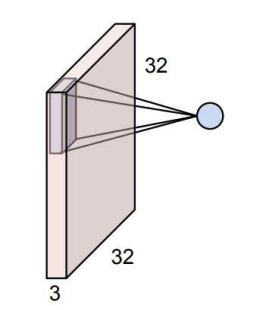
\includegraphics[keepaspectratio, scale=0.7]{pic/img2.png}
		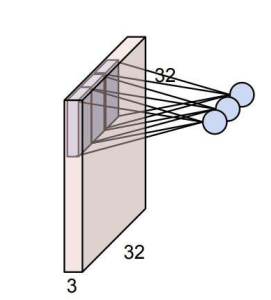
\includegraphics[keepaspectratio, scale=0.7]{pic/img3.png}
		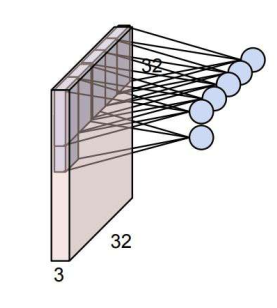
\includegraphics[keepaspectratio, scale=0.7]{pic/img4.png}	
		
	\end{frame}
	\begin{frame}{Convolution process (2)}
		\centering
		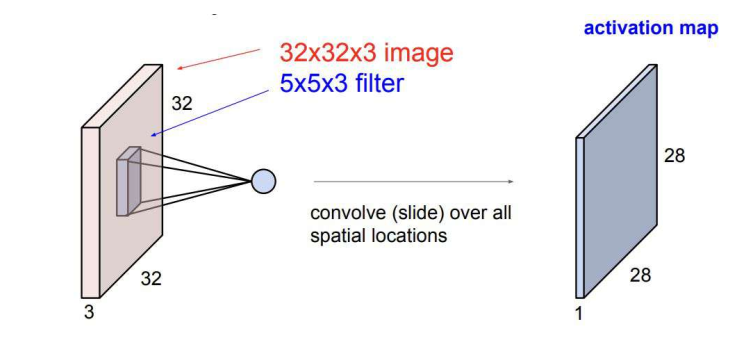
\includegraphics[keepaspectratio, scale=0.75]{pic/img5.png}
		\smallskip
		\begin{flushleft}
			If we consider the \textcolor{red}{image} to be of size \textcolor{blue}{\( n \times m \times b \)} and the \textcolor{red}{filter} to be of size \textcolor{blue}{\( n' \times m' \times b \)}, we will have an \textcolor{red}{activation map} of size \textcolor{blue}{\( (n - n' + 1) \times (m - m' + 1) \times 1 \)} for each filter.
		\end{flushleft}
		
	\end{frame}
	\begin{frame}{Convolution process (3)}
		\centering
		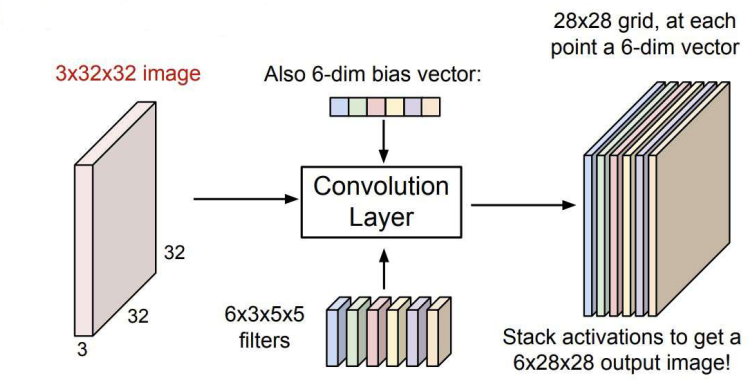
\includegraphics[keepaspectratio, scale=0.8]{pic/img6.png}
	\end{frame}
	\begin{frame}{Convolution process (4)}
		\centering
		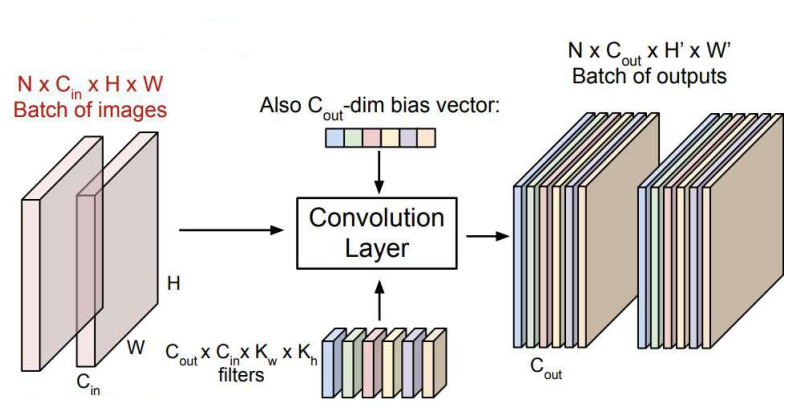
\includegraphics[keepaspectratio, scale=0.7]{pic/img7.png}
		\smallskip
		\begin{flushleft}
			Batching input images can provide a more generalized representation, as described above.
		\end{flushleft}		
	\end{frame}
	\begin{frame}{A different view}
		\centering
		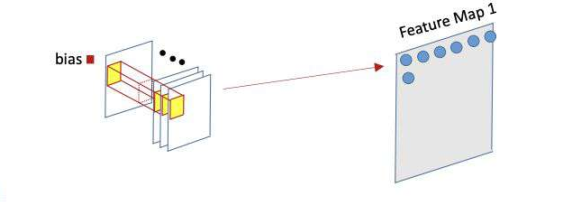
\includegraphics[keepaspectratio, scale=0.9]{pic/diff_view.png}
		
		
		\[ z(i,j,s) = \underbrace{\sum_p \underbrace{\sum_{k=1}^{L} \sum_{l=1}^{L} w(k,l,p,s) a(i+l-1, j+k-1, p)}_{\text{One map}}}_{\text{All maps}} + b(s) \]
		
	\end{frame}
	\begin{frame}{Stride (1)}
		\centering
		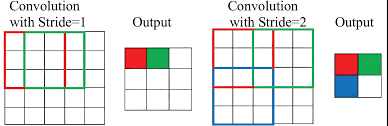
\includegraphics[keepaspectratio, scale=0.9]{pic/stride.png}
		\begin{itemize}
			\item The scans of the individual ``filters'' may advance by more than one pixel at a time
			\begin{itemize}
				\item The ``stride'' may be greater than 1
				\item Effectively increasing the granularity of the scan
				\begin{itemize}
					\item Saves computation, sometimes at the risk of losing information
				\end{itemize}
			\end{itemize}
			\item This results in a reduction in the size of the resulting maps
			\begin{itemize}
				\item They will shrink by a factor equal to the stride
			\end{itemize}
			\item This can happen at any layer
		\end{itemize}
	\end{frame}
	\begin{frame}{Stride (2)}
		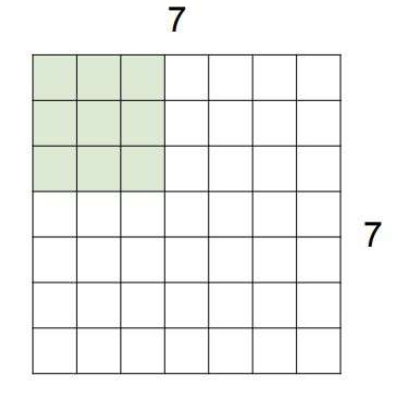
\includegraphics[keepaspectratio, scale=0.5]{pic/stride11.png}
		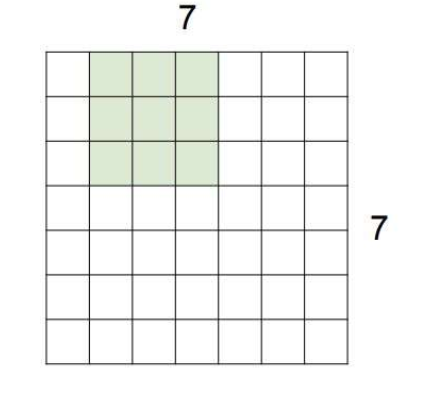
\includegraphics[keepaspectratio, scale=0.5]{pic/stride12.png}
		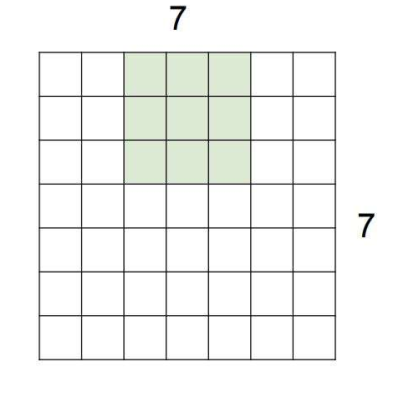
\includegraphics[keepaspectratio, scale=0.5]{pic/stride13.png}
		
		\smallskip	
		\begin{itemize}
			\item Stride: 1
			\item output dimension : 5 $\times$ 5
		\end{itemize}
	\end{frame}
	\begin{frame}{Stride (3)}
		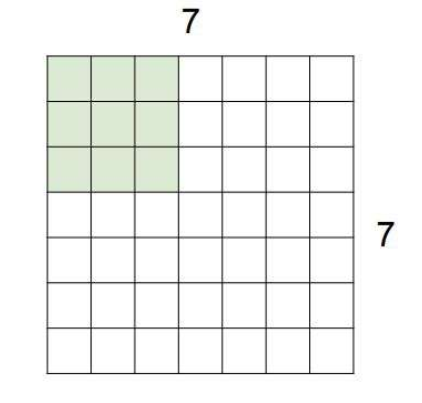
\includegraphics[keepaspectratio, scale=0.5]{pic/stride21.png}
		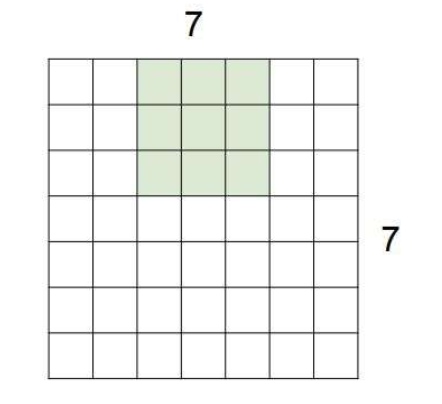
\includegraphics[keepaspectratio, scale=0.5]{pic/stride22.png}
		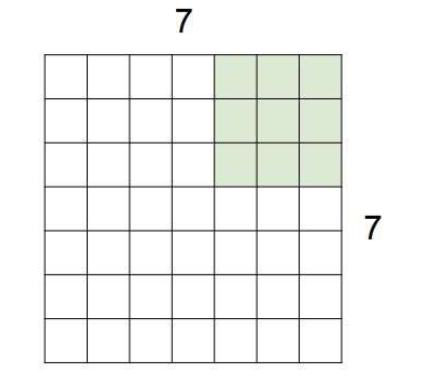
\includegraphics[keepaspectratio, scale=0.5]{pic/stride23.png}
		
		\smallskip	
		\begin{itemize}
			\item stride : 2
			\item output dimension : 3 $\times$ 3
		\end{itemize}
	\end{frame}
	\begin{frame}{Stride (4)}
		\centering
		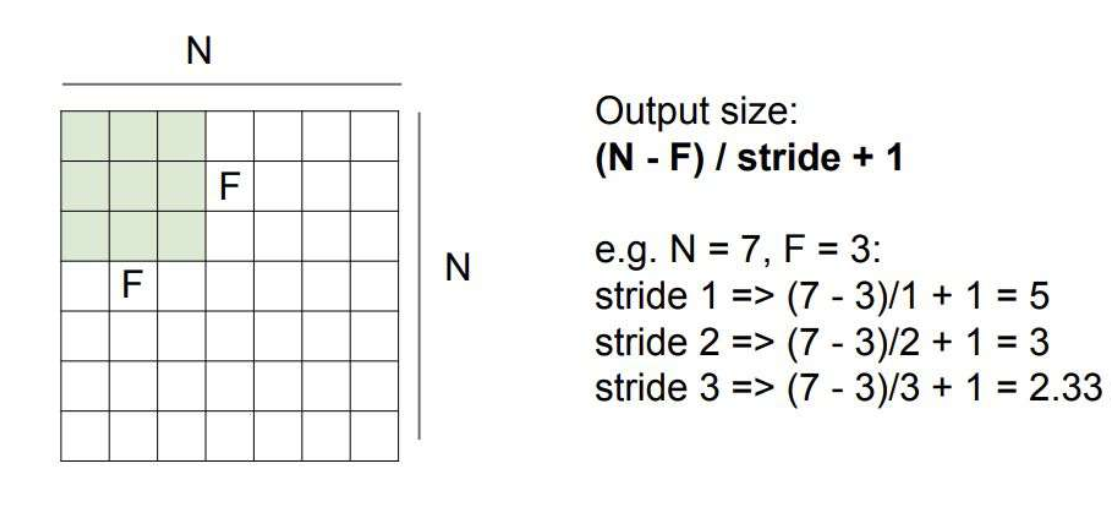
\includegraphics[keepaspectratio, scale=0.5]{pic/strideComp.png}
		\smallskip		
		\begin{itemize}
			\item We can't choose any stride blindly!
			\item The output dimensions must be integers.
			\item This is why padding comes into the picture.
		\end{itemize}
		
	\end{frame}
	\begin{frame}{Padding (1)}
		
		\begin{minipage}{0.28\textwidth} % Adjust width to your liking
			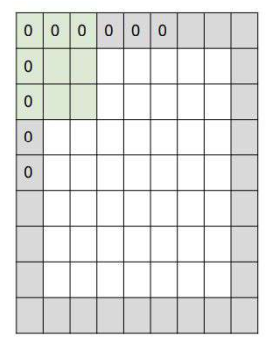
\includegraphics[keepaspectratio, scale=0.6]{pic/zeropad.png}
		\end{minipage}
		\begin{minipage}{0.67\textwidth} % Adjust width to your liking
			In practice, it is common to zero-pad the border.
			\smallskip
			\textbf{Recall:} The original formula for convolution without padding:
			\[
			\frac{N - F}{\text{stride}} + 1
			\]
			
			Now, we should adjust the formula considering padding $P$:
			\[
			\frac{N + 2P - F}{\text{stride}} + 1
			\]
		\end{minipage}
	\end{frame}
	\begin{frame}{Padding (2)}
		\begin{itemize}
			\item Zero-padding is used not only for stride $> 1$, but also to prevent a reduction in output size even when $S = 1$.
			
			\item For stride $> 1$, zero padding is adjusted to ensure that the size of the convolved output is $\left\lceil \frac{N}{S} \right\rceil$
			\\
			This is achieved by zero padding the image with  $ P = S\left\lceil \frac{N}{S} \right\rceil - N$
			
			\item For an $F$ width filter:
			\begin{itemize}
				\item \textbf{Odd $F$}: Pad on both left and right with $\frac{F-1}{2}$ columns of zeros
				\item \textbf{Even $F$}: Pad one side with $\frac{F}{2}$ columns of zeros, and the other with $\frac{F}{2} - 1$ columns of zeros
				\item The resulting image is width $N + F - 1$
			\end{itemize}
			\item The top/bottom zero padding follows the same rules to maintain map height after convolution
			
		\end{itemize}
	\end{frame}
	\begin{frame}{Convnet (1)}
		\centering
		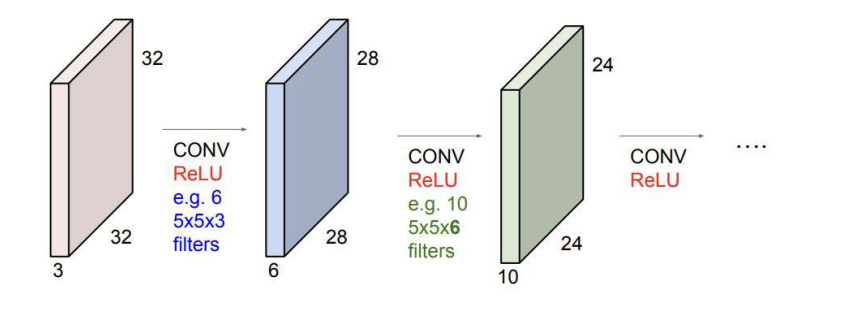
\includegraphics[keepaspectratio, scale=0.7]{pic/convnet.png}
		\smallskip
		\begin{itemize}
			\item \textbf {ConvNet:} sequence of convolution layers, \textcolor{red}{interspersed with activation functions.}
		\end{itemize}
	\end{frame}
	\begin{frame}{Convnet (2)}
		\textbf{Question:}
		What do convolutional filters at different levels of a ConvNet learn?
		
		\bigskip
		
		\textbf{Answer:} 
		\begin{itemize}
			\item Filters in the early layers typically detect simple features, such as edges, textures, and basic shapes.
			\item As we move deeper into the network, the filters learn more complex and abstract features, such as specific parts of objects (e.g., a nose, eyes, or other high-level patterns).
		\end{itemize}
	\end{frame}
	\begin{frame}{Example-1}
		\textbf{Input volume:} \textcolor{blue}{32x32x3}\\
		\textcolor{red}{10} \textcolor{purple}{5x5} filters with stride \textcolor{deepgreen}{1}, pad \textcolor{purple}{2}\\[10pt]
		
		\textbf{Output volume size:}\\
		\[
		\left(\frac{32 + 2 \times 2 - 5}{1}\right) + 1 = 32 \text{ spatially, so} \ \textcolor{blue}{32x32x}\textcolor{red}{10}
		\]
	\end{frame}
	\begin{frame}{Example-2}
		
		\textbf{Input volume:} \textcolor{blue}{32x32x3}\\
		\textcolor{red}{10} \textcolor{purple}{5x5} filters with stride \textcolor{deepgreen}{1}, pad \textcolor{purple}{2}\\[10pt]
		
		\textbf{How many parameters are in this layer?}\\
		Each filter has \textcolor{purple}{5*5}*\textcolor{orange}{3} + 1 = \textcolor{deepgreen}{76} params \hspace{5pt} \textit{(+1 for bias)}\\
		$\Rightarrow$ \textcolor{deepgreen}{76}*\textcolor{red}{10} = \textbf{760}
	\end{frame}
	\begin{frame}{Parameter setting (1)}
		\begin{minipage}{0.50\textwidth} % Left side for general info
			\begin{itemize}
				\item Accepts a volume of size $W_1 \times H_1 \times D_1$
				\item Requires four hyper-parameters:
				\begin{itemize}
					\item Number of filters $K$
					\item Their spatial extent $F$
					\item The stride $S$
					\item The amount of zero padding $P$
				\end{itemize}
				
				\item Produces a volume of size $W_2 \times H_2 \times D_2$ where:
				\begin{itemize}
					\item $W_2 = \left( \frac{W_1 - F + 2P}{S} \right) + 1$
					\item $H_2 = \left( \frac{H_1 - F + 2P}{S} \right) + 1$
					\vspace{2pt}
					\item $D_2 = K$
				\end{itemize}
			\end{itemize}
		\end{minipage}
		\hfill % Horizontal space between the two minipages
		\begin{minipage}{0.45\textwidth} % Right side for common settings
			\textbf{Common settings:}
			\begin{itemize}
				\item $K =$ powers of 2 (e.g., 32, 64, \dots)
				\item $F = 3$, $S = 1$, $P = 1$
				\item $F = 5$, $S = 1$, $P = 2$
				\item $F = 5$, $S = 2$, $P = $ whatever fits!
				\item $F = 1$, $S = 1$, $P = 0$
			\end{itemize}
		\end{minipage}
	\end{frame}
	\begin{frame}{Parameter setting (2)}
		\begin{itemize}
			\item With parameter sharing, it introduces $F \cdot F \cdot D_1$ weights per filter, for a total of $(F \cdot F \cdot D_1) \cdot K$ weights and $K$ biases.
			\item In the output volume, the $d$-th depth slice (of size $W_2 \times H_2$) is the result of performing a valid convolution of the $d$-th filter over the input volume with a stride of $S$, and then offset by the $d$-th bias.
		\end{itemize}
	\end{frame}
	\section{Pooling}
	\begin{frame}{Review}
		\textbf{Three Main Types of Layers}
		\begin{itemize}
			\item \textbf{Convolutional Layer}
			\begin{itemize}
				\item Output of neurons are connected to local regions in the input.
				\item Applying the same filter across the entire image.
				\item CONV layer’s parameters consist of a set of learnable filters.
			\end{itemize}
			\item \textbf{Pooling Layer}
			\begin{itemize}
				\item Performs a downsampling operation along the spatial dimensions.
			\end{itemize}
			\item \textbf{Fully-Connected Layer}
			\begin{itemize}
				\item Typically used in the final stages of the network to combine high-level features and make predictions.
			\end{itemize}
		\end{itemize}
	\end{frame}
	\begin{frame}{Pooling (1)}
		\centering
		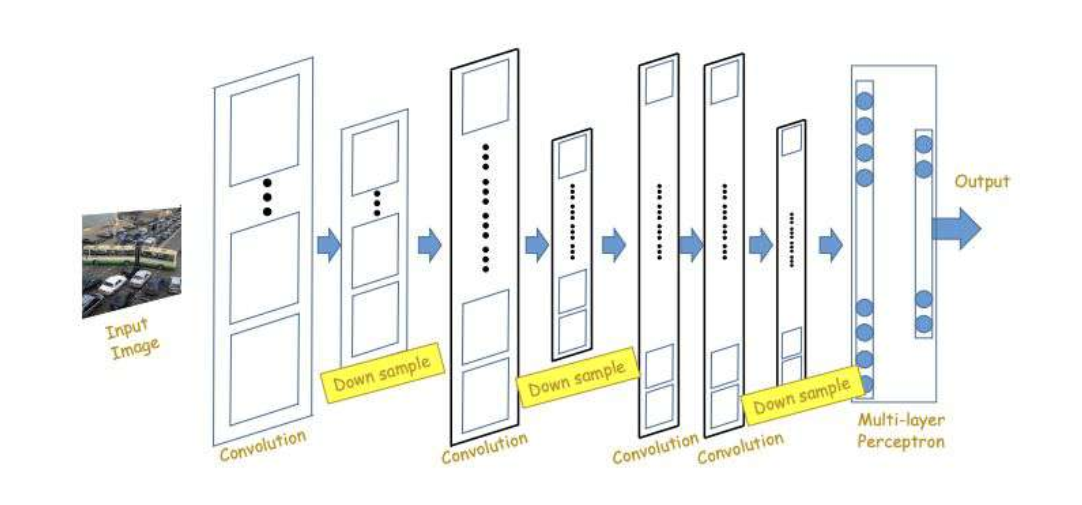
\includegraphics[keepaspectratio, scale=0.5]{pic/pooling.png}
		\smallskip
		\begin{flushleft}
			Convolution \& activation layers are followed intermittently by pooling layers.
			\begin{itemize}
				\item Often, they alternate with convolution, though this is not necessary.
			\end{itemize}
		\end{flushleft}
	\end{frame}
	\begin{frame}{Pooling (2)}
		\centering 
		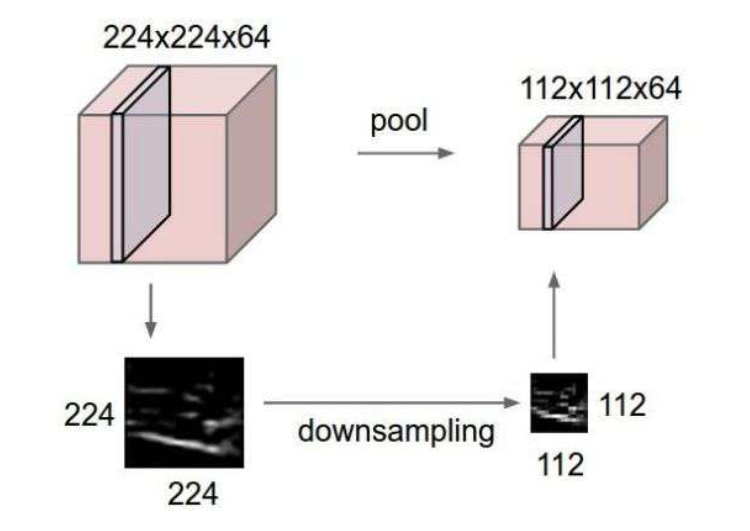
\includegraphics[keepaspectratio, scale=0.4]{pic/pooling1.png}
		\smallskip
		\begin{itemize}
			\item Reduce the spatial size of the representation.
			\begin{itemize}
				\item To reduce the number of parameters and computational demands within the network.
				\item To control overfitting.
			\end{itemize}
			\item Help the network to become invariant to small translations or distortions.
			\item Operates over each activation map independently.
		\end{itemize}
		
	\end{frame}
	\begin{frame}{Pooling (3)}
		\centering
		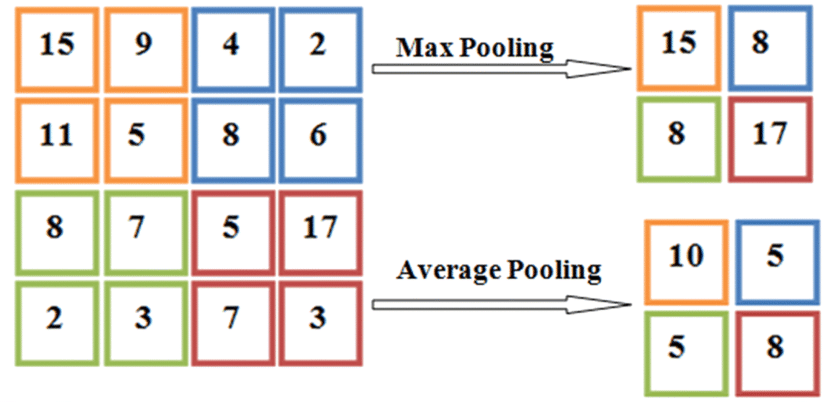
\includegraphics[keepaspectratio, scale=0.6]{pic/pooling2.png}
		\begin{flushleft}
			\textbf{Two Primary Types of Pooling:}
			\begin{itemize}		
				\item \textbf{Max Pooling:}  Selects the maximum value from each patch of the feature map.
				\item \textbf{Average Pooling:} Computes the average of the values in each patch of the feature map.
			\end{itemize}
		\end{flushleft}
	\end{frame}
\begin{frame}{Parameter setting (1)}
	\textbf{Question:} \\
	How does a pooling layer affect the dimensions of the input image?
	
	\bigskip
	
	\textbf{Answer:} \\
	\begin{itemize}
		\item An $N \times N$ picture compressed by a $P \times P$ pooling filter with stride $S$ results in an output map of side $\left\lceil \frac{(N - P)}{S} \right\rceil + 1$.
		\item Typically, pooling layers do not use zero-padding.
	\end{itemize}
\end{frame}

	\begin{frame}{Parameter setting (2)}
		\begin{itemize}
			\item Pooling accepts a volume of size $W_1 \times H_1 \times D_1$
			\item Requires two hyperparameters:
			\begin{itemize}
				\item Their spatial extent $F$,
				\item The stride $S$.
			\end{itemize}
			\item Produces a volume of size $W_2 \times H_2 \times D_2$ where:
			\begin{itemize}
				\item $W_2 = \frac{(W_1 - F)}{S} + 1$
				\item $H_2 = \frac{(H_1 - F)}{S} + 1$
				\item $D_2 = D_1$
			\end{itemize}
			\item Introduces zero parameters since it computes a fixed function of the input.
			\item It is uncommon to use zero-padding for pooling layers.
		\end{itemize}
	\end{frame}
	\begin{frame}{Alternative to pooling}
		\centering
		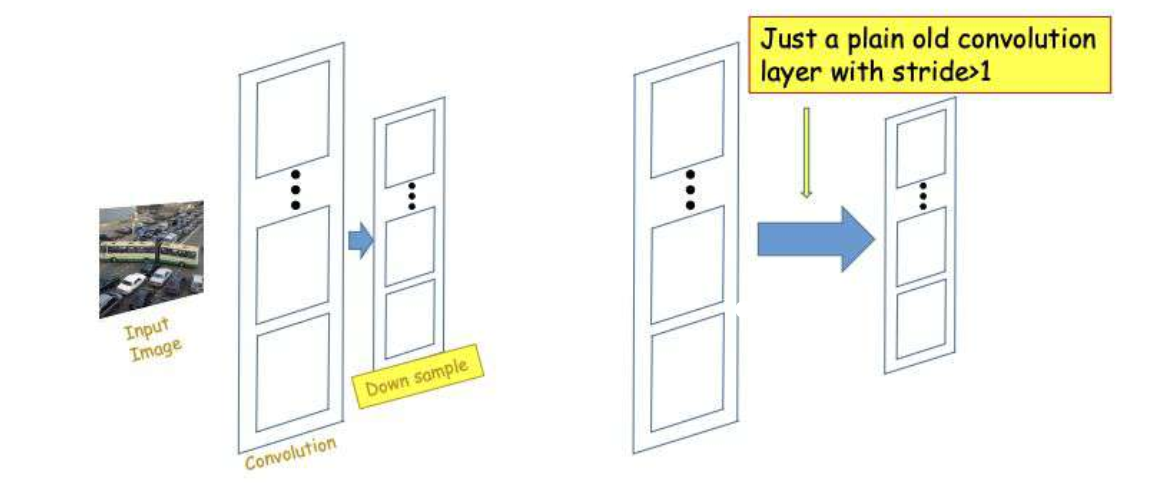
\includegraphics[keepaspectratio, scale=0.55]{pic/pooling3.png}
		\smallskip
		\begin{flushleft}
			Downsampling  be done by a simple convolution layer with stride larger than 1, Replacing the max pooling layer with a convolution layer.
		\end{flushleft}
	\end{frame}
	\begin{frame}{Receptive field (1)}
		\centering
		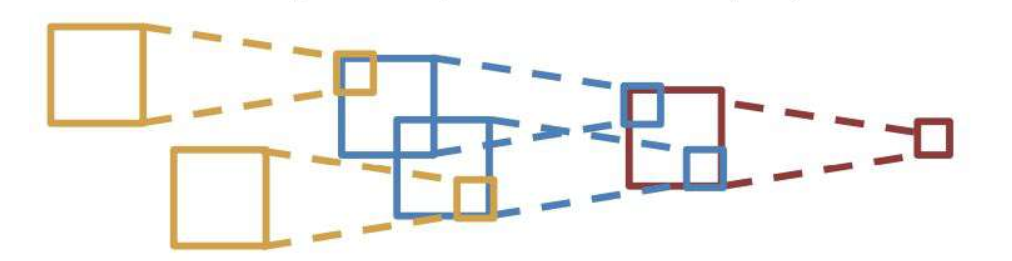
\includegraphics[keepaspectratio, scale=0.6]{pic/receptive1.png}
		\smallskip
		\begin{itemize}
			\item \textbf{Receptive Field :} How big of a region in the \textcolor{red}{input or previous} layer does a neuron on the n-th conv-layer see?
			\item For convolution with kernel size $K$, each element in the next layer depends on a $K \times K$ \textbf{receptive field} in the previous layer.
		\end{itemize}
	\end{frame}	
	\begin{frame}{Receptive field (2)}
		\centering
		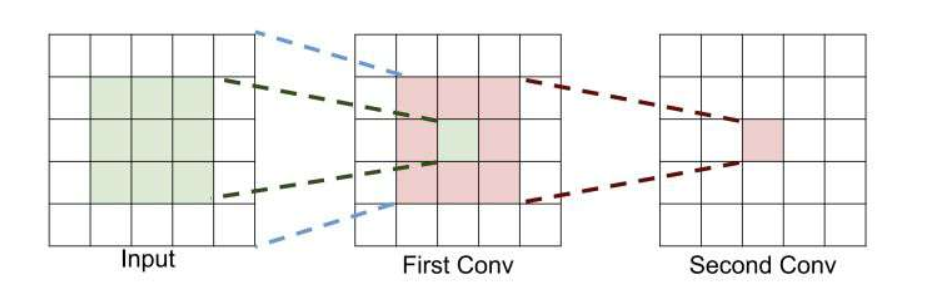
\includegraphics[keepaspectratio, scale=0.6]{pic/receptive.png}
		\smallskip
		\begin{itemize}
			\item Units in the deeper layers can be \textcolor{red}{indirectly} connected to most of the input image.
			\item Each successive convolution adds $K - 1$ to the receptive field size. With $L$ layers, the receptive field size is $1 + L \cdot (K - 1)$.
			\item \textcolor{red}{\textbf{Problem:}} For large images, we need many layers for each output to "see" the whole image.
			\begin{itemize}
				\item \textcolor{red}{\textbf{Solution:}} Downsample inside the network using strides and pooling.
			\end{itemize}
		\end{itemize}
	\end{frame}
	\begin{frame}{Power of small filters}
		Suppose the input is $H \times W \times C$ and we use convolutions with $C$ filters to preserve depth (stride 1, padding to preserve $H, W$).
		
		\bigskip
		\begin{minipage}{0.45\textwidth}
			\textcolor{blue}{\textbf{one CONV with 7 x 7 filters}} \\
			Number of weights \\
			$= C \times (7 \times 7 \times C) = \textbf{49} C^2$
		\end{minipage}
		\hfill
		\begin{minipage}{0.45\textwidth}
			\textcolor{red}{\textbf{three CONV with 3 x 3 filters}} \\
			Number of weights \\
			$= 3 \times C \times (3 \times 3 \times C) = \textbf{27} C^2$
		\end{minipage}
		\bigskip
		\begin{flushleft}
			Both options achieve a receptive field of 7; however, using multiple smaller filters reduces the number of parameters, introduces more nonlinearity, and generally leads to a more efficient, expressive model.
		\end{flushleft}
	\end{frame}
	\section{Inductive bias \& Receptive field}
	
	
	% Slide 1: Inductive Bias in CNNs
	\begin{frame}{Inductive bias in CNNS}
		\textbf{Inductive Bias:} \\
		Refers to the assumptions a model incorporates to generalize from training data to unseen data.
		
		\bigskip
		\textbf{Key Features of Inductive Bias in CNNs:}
		\begin{itemize}
			\item \textbf{Weight Sharing:} \\
			A single filter is applied across different regions of the input, significantly reducing the number of parameters.
			
			\item \textbf{Locality:} \\
			CNNs use small filters (e.g., $3 \times 3$) that focus on local regions, aligning well with image data where local structures are important.
			
			\item CNNs are more sample-efficient than FCNs due to their inductive biases.
			\item CNNS reduce sample complexity from $O(d^2)$ in FCNs to $O(\log^2 d)$.
		\end{itemize}
	\end{frame}
	
	
	\section{Backpropagation}
	\begin{frame}{Summary of concepts}
		\centering
		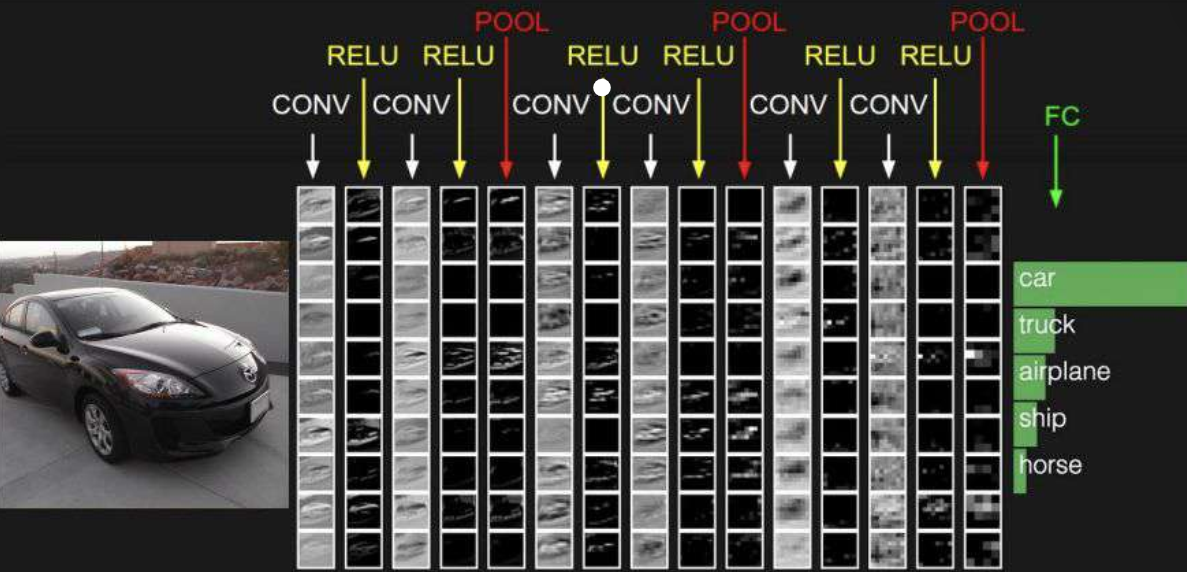
\includegraphics[keepaspectratio, scale=0.65]{pic/car.png}
	\end{frame}
	
	\begin{frame}{Training (1)}
		\centering
		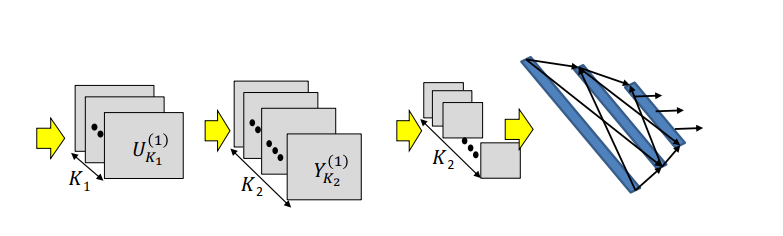
\includegraphics[keepaspectratio, scale=0.6]{pic/training.png}
		\smallskip
		\begin{itemize}
			\item Training is as in the case of the regular MLP
			\item Training examples of (Image, class) are provided
			\item The difference between the desired and actual network output for any input
			\item \textbf{Network parameters are optimized using gradient descent variants}
			\item \textbf{Gradients are computed through backpropagation}
		\end{itemize}
	\end{frame}
	\begin{frame}{Training (2)}
		\centering
		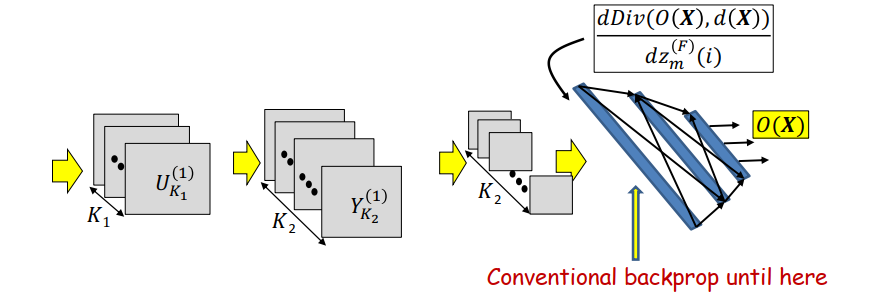
\includegraphics[keepaspectratio, scale=0.6]{pic/training1.png}
		\smallskip
		\begin{itemize}
			\item Backpropagation continues in the usual manner until the computation of the derivative of the divergence w.r.t the inputs to the first ``flat'' layer
		\end{itemize}
		
	\end{frame}
	\begin{frame}{Training (3)}
		
		\centering
		\includegraphics[keepaspectratio, scale=0.6]{pic/training2.png}
		\smallskip
		
		\begin{itemize}
			\item Backpropagation from the flat MLP requires special consideration of:
			\begin{itemize}
				\item The pooling layers, particularly Maxout
				\item The shared computation in the convolution layers
			\end{itemize}
			
			
		\end{itemize}
		
		
	\end{frame}
	\begin{frame}{Backpropagation maxout (1)}
		\centering
		\includegraphics[keepaspectratio, scale=0.6]{pic/training3.png}
		\smallskip
		
		\begin{itemize}
			\item The derivative w.r.t \textcolor{red}{\( U^{(n)}_m (i,j) \)} can be computed via backprop.
			\item But this cannot be propagated backwards to compute the derivative w.r.t. \textcolor{blue}{\( Y^{(n)}_m (k,l) \)}.
			\item \textcolor{red}{\textbf{Max and argmax are not differentiable.}}
		\end{itemize}
		
	\end{frame}
	\begin{frame}{Backpropagation maxout (2)}
		\centering
		\includegraphics[keepaspectratio, scale=0.6]{pic/training4.png}
		\smallskip
		
		\begin{itemize}
			\item \[
			\frac{dDiv(O(X), d(X))}{dY^{(n)}_m (k,l)} = 
			\begin{cases} 
				\frac{dDiv(O(X), d(X))}{dU^{(n)}_m (i,j)} & \text{if } (k,l) = P^{(n)}_m (i,j) \\
				\textcolor{red}{0} & \text{otherwise}
			\end{cases}
			\]
			\item \textbf{Approximation:} Derivative w.r.t the \textcolor{blue}{Y} terms that did not contribute to the maxout map is 0.
		\end{itemize}
		
	\end{frame}
	\begin{frame}{Backpropagation weights}
		\centering
		\includegraphics[keepaspectratio, scale=0.6]{pic/training5.png}
		\smallskip
		
		\begin{itemize}
			\item \textbf{Note:} each weight contributes to \textit{every} position in the map at the output of the convolutional layer.
			\item \textcolor{red}{\textbf{Every position will contribute to the derivative of the weight}}
			\begin{itemize}
				\item \textcolor{red}{Updating shared parameters}
				
			\end{itemize}
		\end{itemize}
		
		
	\end{frame}
	
	
	
	\begin{frame}{Learning the network}
		\centering
		\includegraphics[keepaspectratio, scale=0.6]{pic/training6.png}
		\smallskip
		
		\begin{itemize}
			\item Derived the divergence concerning every intermediate output and free parameter (filter weights).
			\item Can now be embedded in the gradient descent framework to learn the network.
		\end{itemize}
		
		
		
	\end{frame}	
	
	\begin{frame}{A problem}
		
		\centering
		\includegraphics[keepaspectratio, scale=0.6]{pic/training7.png}
		\smallskip
		
		
		
		\begin{flushleft}
			\textbf{Question:} How can generalization be improved?
			\bigskip
			\textbf{Answer:} Rotation, Translation, Rescaling, Flipping, etc.
			
		\end{flushleft}
		
	\end{frame}
	\begin{frame}{Design choices}
		
		\begin{itemize}
			\item \textbf{Number of convolutional and downsampling layers}
			\begin{itemize}
				\item Arrangement (order in which they follow each other)
			\end{itemize}
			
			\item \textbf{For each convolutional layer:}
			\begin{itemize}
				\item Number of filters $d^l$
				\item Spatial extent of filter $F^l \times F^l$
				\begin{itemize}
					\item The "depth" of the filter is fixed by the number of filters in the previous layer $d^{l-1}$
				\end{itemize}
				\item The stride $S^l$
			\end{itemize}
			
			\item \textbf{For each downsampling or pooling layer:}
			\begin{itemize}
				\item Spatial extent of filter $P^l \times P^l$
				\item The stride $S^l$
			\end{itemize}
			
			\item \textbf{For the final multi-layer perceptron (MLP):}
			\begin{itemize}
				\item Number of layers, and number of neurons in each layer
			\end{itemize}
			
		\end{itemize}
		
	\end{frame}
	
	
	\begin{frame}{Typical architecture for CNNS}
		
		\begin{itemize}
			\item \texttt{[(CONV-RELU)*N – POOL?]*M – (FC-RELU)*K – SOFTMAX}
			\begin{itemize}
				\item Where N is usually up to $\sim 5$
				\item M is a large number
				\item $0 \leq K \leq 2$
			\end{itemize}
		\end{itemize}
		
		\bigskip
		
		\textbf{But recent advances such as ResNet and GoogleNet challenge this paradigm!}
		
	\end{frame}
	
	
	\begin{frame}{Conclusion}
		
		\begin{itemize}
			\item Highly structured nature of image data
			\item Local correlations are important
			\item CNNs have local and shared connections
			\item CNNs introduce strong inductive biases
			\item To leverage the two-dimensional structure of image data and introduce inductive biases, four interrelated concepts can be used:
			\begin{itemize}
				\item Hierarchy
				\item Locality
				\item Invariance 
			\end{itemize}
		\end{itemize}
		
	\end{frame}
	
	\section{References}
	\begin{frame}
		content...
	\end{frame}
	
	
	
\end{document}